William Grey Walter nació en Kansas (EE.UU.) en 1910 y se trata de uno de los pioneros en el campo de la robótica, cibernética e inteligencia artificial. Sus estudios en neurología le llevaron a la investigación y desarrollo de inventos que eran capaces de medir ondas cerebrales y analizar el comportamiento del cerebro de una persona. Más concretamente, con la idea de que la conexión de neuronas o células cerebrales se podían ejecutar comportamientos complejos. Esto dio lugar a la construcción en 1948 y 1949 de las \textit{tortugas} Elmer y Elsie, respectivamente.\\

El nombre de tortugas se debe al caparazón de plástico que protegía al robot además de su lentitud en los movimientos. Solo estaban programadas para hacer dos misiones; esquivar obstáculos aunque no de una forma muy inteligente y volver a recargar su batería cuando esta estuviera cerca de agotarse. Las tortugas estaban formado por tres ruedas, una batería y una célula fotoeléctrica móvil que actuaba sobre el motor para decidir la dirección de los movimientos como lo hacen los actuales sensores.

\begin{figure}[H]
\begin{center}
  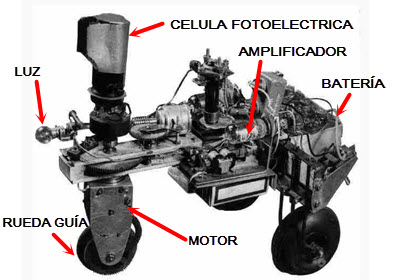
\includegraphics[width=0.5\textwidth]{./EtapaPrimeriza/imagenes/t1.jpg}
  \caption{Estructura de las Tortuga autónomas (\href{https://vonneumannmachine.files.wordpress.com/2011/05/elsie.jpg} {Von Neumann})}
  \label{t1}
\end{center}
\end{figure}


Walter fue el precursor de los robot aspiradores están tan de moda en nuestros días y que nos facilitan notablemente las tareas del hogar.
